\documentclass[aspectratio=169, 10pt]{beamer}

% ==============================================================================
% THEME & STYLING CONFIGURATION
% ==============================================================================

\usetheme{Madrid}
\usecolortheme{whale}

% Custom Colors
\definecolor{primaryblue}{RGB}{15, 76, 129}
\definecolor{accentteal}{RGB}{0, 150, 136}
\definecolor{darkslate}{RGB}{30, 41, 59}

\definecolor{alertred}{RGB}{220, 38, 38}
\definecolor{successgreen}{RGB}{16, 185, 129}

\setbeamercolor{palette primary}{bg=primaryblue, fg=white}
\setbeamercolor{structure}{fg=primaryblue}
\setbeamercolor{title}{bg=primaryblue, fg=white}
\setbeamercolor{frametitle}{bg=primaryblue, fg=white}
\setbeamercolor{block title}{bg=primaryblue!15, fg=primaryblue}
\setbeamercolor{block body}{bg=primaryblue!5, fg=darkslate}
\setbeamercolor{block title alerted}{bg=alertred!15, fg=alertred}
\setbeamercolor{block body alerted}{bg=alertred!5, fg=darkslate}
\setbeamercolor{block title example}{bg=successgreen!15, fg=successgreen}
\setbeamercolor{block body example}{bg=successgreen!5, fg=darkslate}

\setbeamertemplate{navigation symbols}{}
\setbeamertemplate{itemize items}[circle]
\setbeamertemplate{enumerate items}[default]

% ==============================================================================
% PACKAGES
% ==============================================================================

\usepackage{booktabs}
\usepackage{tabularx}
\usepackage{multicol}
\usepackage{amsmath, amssymb}
\usepackage{listings}
\usepackage{tikz}
\usetikzlibrary{arrows.meta, positioning, shapes.geometric}

% Python Code Highlighting
\lstset{
    language=Python,
    basicstyle=\ttfamily\scriptsize,
    keywordstyle=\color{primaryblue}\bfseries,
    stringstyle=\color{accentteal},
    commentstyle=\color{gray}\itshape,
    breaklines=true,
    showstringspaces=false,
    frame=single,
    rulecolor=\color{gray!30},
    backgroundcolor=\color{gray!5}
}

% ==============================================================================
% TITLE INFORMATION
% ==============================================================================

\title[SENTINEL-Vision]{SENTINEL-Vision: Agent Risk Grounding \& Visual Risk Inspection}
\subtitle{Spatiotemporal Safety Guardrails for Autonomous GUI Agents}

\author[Yugendhar S]{
    \textbf{Yugendhar S} \quad (\texttt{Lead Developer}) \\
    \textbf{Project Team}
}

\institute[University]{
    Department of Artificial Intelligence \& Data Science \\
}

\date{\today}

% ==============================================================================
% PRESENTATION
% ==============================================================================

\begin{document}

% ------------------------------------------------------------------------------
% SLIDE 1: TITLE
% ------------------------------------------------------------------------------

\begin{frame}[plain]
    \titlepage
\end{frame}

% ------------------------------------------------------------------------------
% SLIDE 2: OUTLINE
% ------------------------------------------------------------------------------

\begin{frame}{Presentation Outline}
    \begin{multicols}{2}
        \tableofcontents
    \end{multicols}
\end{frame}

% ==============================================================================
% SECTION 1
% ==============================================================================

\section{Problem Statement \& Motivation}

\begin{frame}{01 $\cdot$ Problem Statement \& Motivation}

    \textbf{Problem Statement:}

    \begin{itemize}
        \item Autonomous GUI agents can execute actions with catastrophic consequences.
        \item Existing safety mechanisms rely on text/code (LLM outputs), ignoring the visual UI context.
        \item We need a visual safety guardrail to predict risks before irreversible actions occur.
    \end{itemize}

    \vspace{0.2cm}

    \begin{columns}[T]

        \begin{column}{0.48\textwidth}

            \begin{alertblock}{Limitation of Existing Systems}
                Text-based safety filters fail to understand what the agent is actually clicking on the screen, leading to "blind" execution of harmful actions.
            \end{alertblock}

        \end{column}

        \begin{column}{0.48\textwidth}

            \begin{block}{Real-World Impact}
                \begin{itemize}
                    \item \textbf{Financial Loss:} Unauthorized payments.
                    \item \textbf{Privacy Breaches:} Sharing sensitive data.
                    \item \textbf{Data Destruction:} Deleting critical files or databases.
                \end{itemize}
            \end{block}

        \end{column}

    \end{columns}

\end{frame}

% ==============================================================================
% SECTION 2
% ==============================================================================

\section{Project Objectives}

\begin{frame}{02 $\cdot$ Project Objectives \& Scope}

    \begin{columns}[T]

        \begin{column}{0.5\textwidth}

            \begin{block}{Primary Objectives}

                \begin{enumerate}
                    \item Develop a multimodal spatiotemporal model (SENTINEL-Vision) to predict UI risks.
                    \item Categorize risks into Destructive, Financial, Privacy, and Irreversible External.
                    \item Localize harmful UI elements using bounding box prediction.
                    \item Implement an asymmetric Decision Gate policy (RL) prioritizing safety.
                \end{enumerate}

            \end{block}

        \end{column}

        \begin{column}{0.48\textwidth}

            \begin{block}{Engineering Deliverables}

                \begin{itemize}
                    \item Preprocessed trajectory datasets (Multimodal-Mind2Web, ScreenSpot).
                    \item ViT-based Spatiotemporal Vision Model.
                    \item PPO-trained Decision Gate Policy.
                    \item Optimized INT8 ONNX models for real-time deployment.
                \end{itemize}

            \end{block}

        \end{column}

    \end{columns}

\end{frame}

% ==============================================================================
% SECTION 3
% ==============================================================================

\section{System Architecture \& Pipeline}

\begin{frame}{03 $\cdot$ System Architecture \& Pipeline}

    \begin{center}

        \resizebox{0.95\textwidth}{!}{
            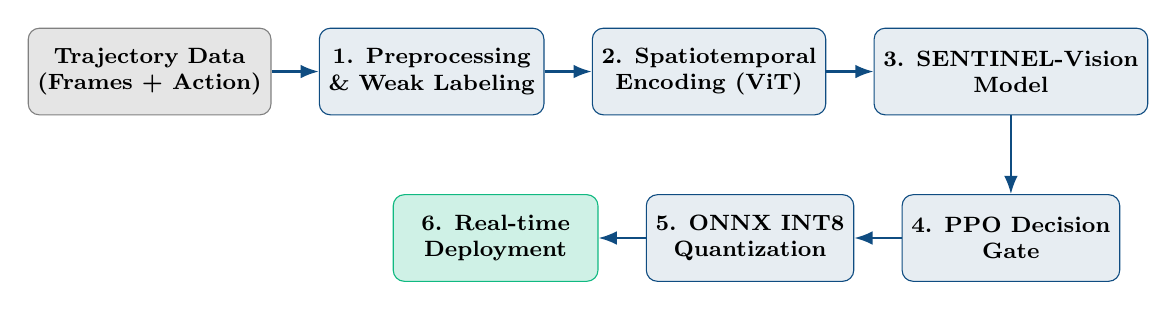
\begin{tikzpicture}[
                node distance=1.1cm,
                box/.style={
                    rectangle,
                    draw=primaryblue,
                    fill=primaryblue!10,
                    rounded corners,
                    text centered,
                    minimum width=2.6cm,
                    minimum height=1.1cm,
                    font=\bfseries\footnotesize,
                    align=center
                },
                arrow/.style={-Latex, thick, primaryblue}
            ]

            % Top Row
            \node (input) [box, fill=gray!20, draw=gray] {Trajectory Data\\(Frames + Action)};

            \node (process1) [box, right=0.6cm of input]
            {1. Preprocessing\\\& Weak Labeling};

            \node (process2) [box, right=0.6cm of process1]
            {2. Spatiotemporal\\Encoding (ViT)};

            \node (process3) [box, right=0.6cm of process2]
            {3. SENTINEL-Vision\\Model};

            % Bottom Row
            \node (process4) [box, below=1.0cm of process3]
            {4. PPO Decision\\Gate};

            \node (process5) [box, left=0.6cm of process4]
            {5. ONNX INT8\\Quantization};

            \node (output) [box, fill=successgreen!20,
            draw=successgreen, left=0.6cm of process5]
            {6. Real-time\\Deployment};

            % Arrows
            \draw [arrow] (input) -- (process1);
            \draw [arrow] (process1) -- (process2);
            \draw [arrow] (process2) -- (process3);
            \draw [arrow] (process3) -- (process4);
            \draw [arrow] (process4) -- (process5);
            \draw [arrow] (process5) -- (output);

            \end{tikzpicture}
        }

    \end{center}

\end{frame}

% ==============================================================================
% SECTION 4
% ==============================================================================

\section{Detailed Methodology \& Algorithms}

\begin{frame}{04 $\cdot$ Methodology}

    \begin{columns}[T]

        \begin{column}{0.33\textwidth}

            \begin{block}{1. Preprocessing}

                \small

                \begin{itemize}
                    \item Frame extraction
                    \item Resizing to 224x224
                    \item Missing-value handling
                    \item Weak labeling for harmful cues
                \end{itemize}

            \end{block}

        \end{column}

        \begin{column}{0.33\textwidth}

            \begin{block}{2. Feature Processing}

                \small

                \begin{itemize}
                    \item Frame windowing (k=6)
                    \item ViT feature extraction
                    \item Temporal fusion (cross-attention)
                    \item Dimensionality reduction
                \end{itemize}

            \end{block}

        \end{column}

        \begin{column}{0.33\textwidth}

            \begin{block}{3. Model Heads}

                \small

                \begin{itemize}
                    \item Binary Risk Score [0,1]
                    \item 5-Class Risk Category
                    \item UI Bounding Box [x, y, w, h]
                    \item Asymmetric Focal Loss
                \end{itemize}

            \end{block}

        \end{column}

    \end{columns}

\end{frame}

\begin{frame}{05 $\cdot$ Algorithm / Mathematical Formulation}

    \begin{columns}[T]

        \begin{column}{0.52\textwidth}

            \begin{block}{Mathematical Model}

                \small

                \textbf{Sentinel Multi-Task Loss:}

                \[
                    \mathcal{L}_{total} = w_r \mathcal{L}_{risk} + w_c \mathcal{L}_{cat} + w_l \mathcal{L}_{loc}
                \]

                \textbf{Asymmetric Focal Loss (Risk):}

                \[
                    \mathcal{L}_{risk} = -\alpha_t (1 - p_t)^\gamma \log(p_t)
                \]

                \textit{Where False Negatives are heavily penalized.}

                \textbf{RL Objective (Decision Gate):}

                Maximize Reward $R(s, a)$ with $-10$ penalty for allowing a harmful action.

            \end{block}

        \end{column}

        \begin{column}{0.46\textwidth}

            \begin{block}{Algorithm Steps}

                \begin{enumerate}
                    \item Input $k$ UI frames + Action.
                    \item Extract ViT spatial embeddings.
                    \item Fuse temporally to capture context.
                    \item Predict Risk, Category, and BBox.
                    \item Pass to RL Decision Gate.
                    \item Allow or Block Agent Action.
                \end{enumerate}

            \end{block}

        \end{column}

    \end{columns}

\end{frame}

% ==============================================================================
% SECTION 5
% ==============================================================================

\section{Datasets \& Preprocessing}

\begin{frame}{06 $\cdot$ Dataset \& Preprocessing}

    \textbf{Dataset Overview (16,726 Trajectory Samples)}

    \begin{table}[]
        \centering
        \small

        \begin{tabularx}{\textwidth}{l l r X}

            \toprule
            \textbf{Dataset} &
            \textbf{Type} &
            \textbf{Records} &
            \textbf{Preprocessing} \\

            \midrule

            Multimodal-Mind2Web & Web Trajectories & ~15,000 & Windowing (k=6), Weak Labeling \\

            ScreenSpot (v1/v2) & Single-Frame UI & ~1,700 & BBox Normalization, Categorization \\

            \bottomrule

        \end{tabularx}

    \end{table}

    \vspace{0.2cm}
    \begin{itemize}
        \item \textbf{Split:} Train = 11,707 | Val = 2,507 | Test = 2,512
        \item \textbf{Note:} Only pixels and weak labels used. No internal agent reasoning traces are provided to the model.
    \end{itemize}

\end{frame}

% ==============================================================================
% SECTION 6
% ==============================================================================

\section{Experimental Results \& Evaluation}

\begin{frame}{07 $\cdot$ Experimental Results}

    \begin{columns}[T]

        \begin{column}{0.58\textwidth}

            \textbf{Performance Comparison (Epoch 30)}

            \begin{table}[]

                \centering
                \scriptsize

                \begin{tabularx}{\textwidth}{
                    @{}l c c >{\raggedright\arraybackslash}X@{}
                }

                    \toprule
                    \textbf{Model Config} &
                    \textbf{Recall} &
                    \textbf{F1} &
                    \textbf{Remarks} \\

                    \midrule

                    Spatial-Only (k=1) & 0.65 & 0.60 & Misses contextual harm \\

                    Temporal (k=6) + CE Loss & 0.78 & 0.75 & Balanced but misses edge cases \\

                    \textbf{SENTINEL-Vision} &
                    \textbf{0.92} &
                    \textbf{0.86} &
                    \textbf{Focal Loss + Decision Gate} \\

                    \bottomrule

                \end{tabularx}

            \end{table}

            \vspace{0.1cm}

            \begin{block}{Key Metrics}

                \begin{itemize}
                    \item Peak Harm Recall: \textbf{0.92}
                    \item Peak Harm F1-Score: \textbf{0.86}
                    \item Category Accuracy: \textbf{0.90}
                    \item Localization IoU@0.5: \textbf{0.75}
                \end{itemize}

            \end{block}

        \end{column}

        \begin{column}{0.40\textwidth}

            \begin{exampleblock}{Key Findings}

                \begin{enumerate}
                    \item Asymmetric Focal Loss significantly reduces False Negatives (critical for safety).
                    \item Temporal windowing (k=6) allows detection of contextual risks.
                    \item PPO Decision Gate learns to reject high-uncertainty predictions.
                \end{enumerate}

            \end{exampleblock}

        \end{column}

    \end{columns}

\end{frame}

% ==============================================================================
% SECTION 7
% ==============================================================================

\section{System Integration}

\begin{frame}[fragile]{08 $\cdot$ System Integration / Demo}

    \begin{alertblock}{Existing System (Text-Only)}

        Agents execute code blindly based on DOM/HTML, failing to see visual overlays, warnings, or mismatched UI states.

    \end{alertblock}

    \vspace{0.3cm}

    \begin{exampleblock}{Proposed System (SENTINEL-Vision)}

        Acts as a visual middleware. Intercepts the action, analyzes the UI frames, and blocks execution if risk is detected.

    \end{exampleblock}

    \vspace{0.3cm}

    \begin{lstlisting}
# SENTINEL-Vision Interceptor
frames = get_recent_frames(k=6)
risk_score, category, bbox = sentinel_model(frames)

action_allowed = decision_gate(risk_score, agent_action)

if not action_allowed:
    raise SafetyViolationError(f"Blocked: {category}")
    \end{lstlisting}

\end{frame}

% ==============================================================================
% SECTION 8
% ==============================================================================

\section{Work Accomplished So Far}

\begin{frame}{09 $\cdot$ Work Accomplished So Far}

    \begin{table}[]

        \centering
        \small

        \begin{tabularx}{\textwidth}{l X c}

            \toprule
            \textbf{Component} &
            \textbf{Implementation Details} &
            \textbf{Status} \\

            \midrule

            Data Pipeline &
            Preprocessed Multimodal-Mind2Web and ScreenSpot &
            \textbf{\color{successgreen}Complete} \\

            Architecture &
            Built ViT + Temporal Fusion + Multi-Head outputs &
            \textbf{\color{successgreen}Complete} \\

            Model Training &
            30-Epoch curriculum training on RTX 4050 GPU &
            \textbf{\color{successgreen}Complete} \\

            RL Decision Gate &
            PPO policy optimized for asymmetric risk &
            \textbf{\color{successgreen}Complete} \\

            Optimization &
            ONNX Export and Dynamic INT8 Quantization &
            \textbf{\color{successgreen}Complete} \\

            Documentation &
            Automated Generation of Markdown \& LaTeX Reports &
            \textbf{\color{successgreen}Complete} \\

            \bottomrule

        \end{tabularx}

    \end{table}

\end{frame}

% ==============================================================================
% SECTION 9
% ==============================================================================

\section{Future Roadmap \& Conclusion}

\begin{frame}{10 $\cdot$ Future Roadmap \& Conclusion}

    \begin{columns}[T]

        \begin{column}{0.5\textwidth}

            \begin{block}{Future Scope}

                \begin{itemize}
                    \item Expand to OS-level agents (Windows/macOS GUI).
                    \item Implement real-time inference on edge devices (NPU/Mobile).
                    \item Integrate Vision-Language Models (VLMs) for deeper context.
                    \item Support custom, user-defined risk profiles.
                \end{itemize}

            \end{block}

        \end{column}

        \begin{column}{0.48\textwidth}

            \begin{exampleblock}{Conclusion}

                \begin{enumerate}
                    \item \textbf{Approach:} A multimodal spatiotemporal model for GUI safety.
                    \item \textbf{Results:} Achieved 92\% harm recall with fast inference (ONNX).
                    \item \textbf{Contribution:} SENTINEL-Vision is a critical step towards safe, deployable autonomous agents in real-world scenarios.
                \end{enumerate}

            \end{exampleblock}

        \end{column}

    \end{columns}

\end{frame}

% ------------------------------------------------------------------------------
% THANK YOU SLIDE
% ------------------------------------------------------------------------------

\begin{frame}[plain]

    \centering

    \vspace{1.5cm}

    {\Huge \textbf{\color{primaryblue}Thank You!}} \\

    \vspace{1.0cm}

    {\large Questions?}

\end{frame}

\end{document}
